\documentclass{article}

\usepackage{amsfonts,relsize,amsmath,amssymb,systeme}
\usepackage{listings}

\usepackage{hyperref}

\usepackage{graphicx}
\graphicspath{ {./images/} }

\usepackage[T1]{fontenc}
\usepackage[polish]{babel}
\usepackage[utf8]{inputenc}
\usepackage{lmodern}
\selectlanguage{polish}
\author{Autor: Zbigniew Królikowski
\\\\\\\\}
\title{ Algorytmy dla Problemów Trudnych Obliczeniowo.\\
Rozwiązanie zadania: \textbf{Potęga hetmanów}
Informatyka 2015/16}


\begin{document}
\maketitle


\vfill

\paragraph{Prowadzący: dr hab. inż. Piotr Faliszewski
\\\\\\\\
}

\newpage

\section{Uwagi}

Moja filozofia zapisu: \textbf{hetmany bijące nie zmieniają miejsca tylko znikają na rzecz zbitego} - taki obraz przyjąłem gdyż łatwiej było go rozpisać, mniej dynamiki. Często zapisuję bicie jako redukcję. Nie zmienia to w żaden sposób istoty algorytmu tylko jego opis, który mógłby być mylący bez tej notki.

\section{Reprezentacja problemu}

Plansza została przedstawiona jako \textbf{graf nieskierowany}, w którym każdy węzeł połączony jest z innymi co najwyżej 8 krawędziami.

\subsection{Zapis wartości hetmanów}

W celach uproszczenia obliczeń wartości są reprezentowane jako wykładniki liczby 2.

\subsection{Krótki słownik moich pojęć - w razie wątpliwości}

\begin{itemize}
\item osie - pion, poziom i skosy
\item hetman widoczny dla hetmana \textit{(zbijalny bezpośrednio, ale bez patrzenia na wykładnik)}
\end{itemize}

\section{Wstępne obserwacje - ogranicznie maksymalnej wartości hetmana}

Na wartość końcową hetmana da się nałożyć pewne ograniczenie:

\textbf{Końcowa wartość hetmana $h$ nie może być wyższa od jego aktualnej wartości $V(h) * 2^n$ gdzie $n$ - liczba hetmanów w pionie, poziomie i na skosach (osiach).}

Jest to łatwo udowodnić - każde bicie skierowane przeciwko hetmanowi podnosi jego wartość dwukrotnie. Bić może być \textit{w najlepszym wypadku} tyle ile hetmanów będących na tych samych osiach co dany hetman.

\begin{figure}[!ht]
  \centering
      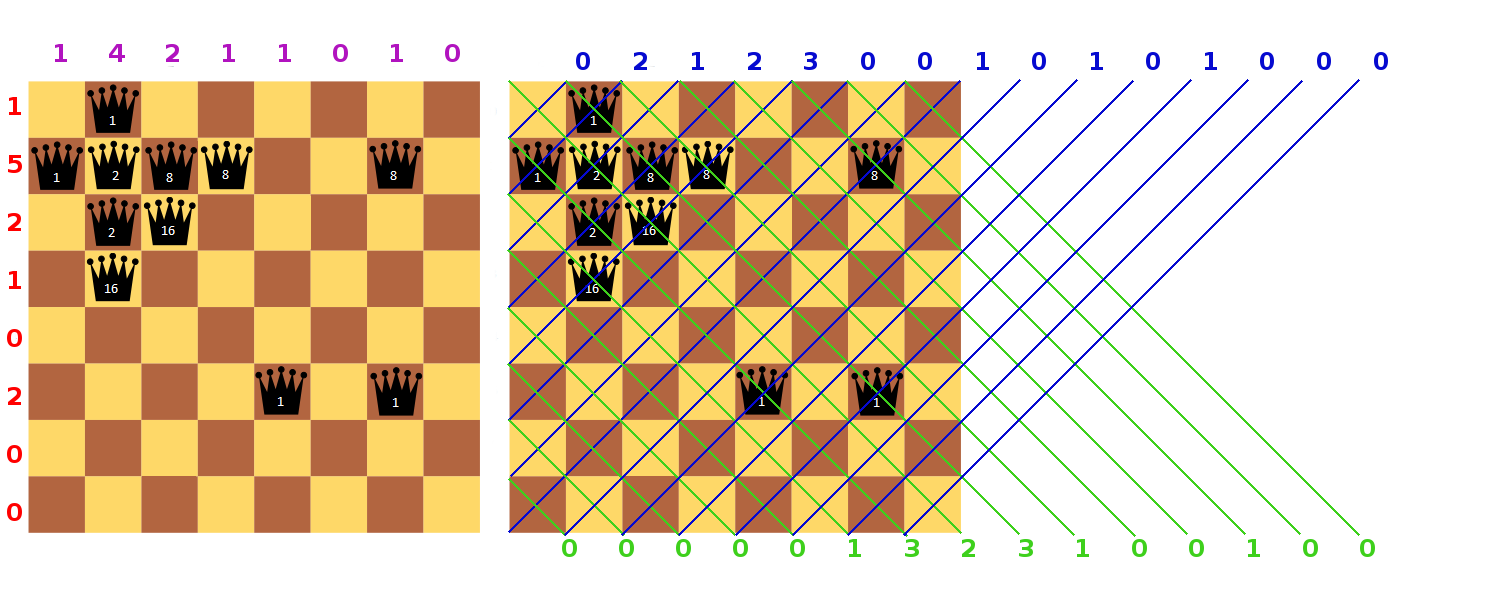
\includegraphics[scale=0.3]{obs1.png}
  \caption{Zliczenie ilości hetmanów na poszczególnych osiach.}
\end{figure}

\begin{figure}[!ht]
  \centering
      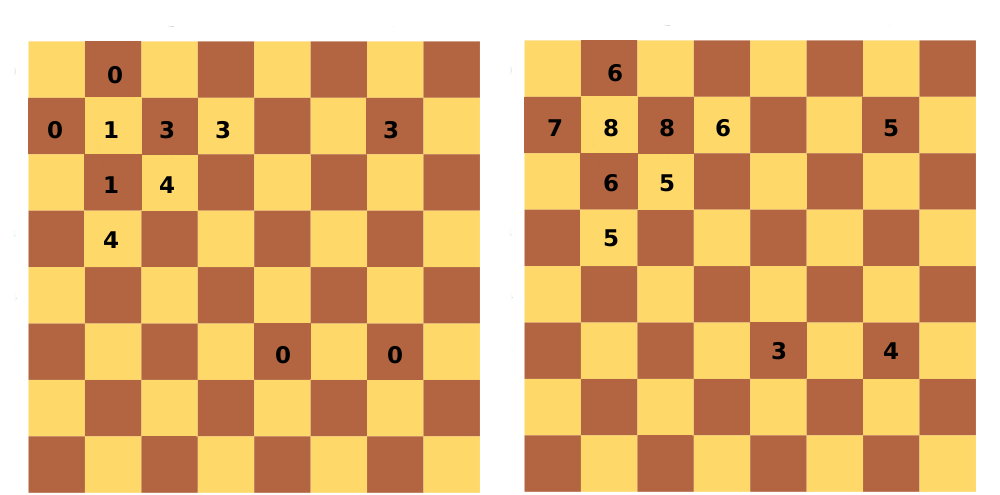
\includegraphics[scale=0.25]{obs1a.png}
  \caption{\textit{Lewo:} Wartość hetmanów w mojej notacji \textit{Prawo:} maksymalna ilość bić skierowana ku konkretnemu hetmanowi.\textit{ Dół:} Górne ograniczenie na wartość końcową hetmanów. Na czerwono hetmany, które nie mogą być końcowe dla K=1.}
  
\end{figure}

Jak zademonstrowano na powyższym przykładzie możemy \textbf{wykluczyć} pewne kombinacje(o wielkości K) hetmanów z bycia końcowymi. Warunkiem wykluczenia jest niemożliwość uzyskania przez tą kombinację wartości będącej sumą wartości wszystkich hetmanów na planszy. Jest to pewne uproszczenie problemu, część postaci rozwiązania.

\paragraph{Bezpośrednio nieużyteczne -}liczba tych kombinacji wynosi $\binom{N} {K}$ gdzie $N$ to liczba hetmanów na planszy a $K$ to ilość hetmanów końcowych.

\subsubsection{Heurystyka}

Możemy się zatem spodziewać, że pewne hetmany zostaną zredukowane "wcześniej niż później", a więc mamy nałożoną jakąś \textbf{kolejność przeszukiwania} przestrzeni rozwiązań. \textbf{Skoro mniejszy potencjał hetmana wiąże się z niemożnością bycia końcowym hetmanem to może powinniśmy ruszać się  wcześniej tymi z mniejszym potencjałem?}

\section{Algorytm}

Algorytm przeszukuje przestrzeń rozwiązań za pomocą wywołań rekurencyjnych modyfikując za każdym razem planszę. Kolejność przeszukiwania jest heurystyką, która zostanie później opisana.

\begin{lstlisting}
//Dane globalne
queens[] // lista hetmanow, kazdy zawiera powiazania do sasiadow
queenCount // obecna liczba hetmanow
targetCount // docelowa liczba hetmanow

bool recursiveCheck():
	if achievedTarget():
		return true
	else:
		sortQueens()
		for queen in board:
			connections = queen.possibleConnections()
			sortConnections()
			for connection in connections:
				move(queen, connection)
				if recursiveCheck():
					return true
	// Nie znaleziono rozwiazania	
		undoMove()	
		return false
		
bool achievedTarget():
	return queenCount <= targetCount

void move(queen, target) // Logika ruchu	
	
\end{lstlisting}

\clearpage

\subsection{Sposób sortowania hetmanów}

\subsubsection{Najprostsze rozwiązanie}

Hetmany porządkujemy w oparciu o wartość:

$$c_n$$
czyli ilość hetmanów "widocznych" \textit{(zbijalnych bezpośrednio, ale bez patrzenia na wykładnik)} z tego pola przed podjęciem jakiegokolwiek ruchu

Algorytm okazał się dawać lepsze wyniki od rozwiązania \textit{brute-force}, zwłaszcza biorąc pod uwagę, że porządek zbijania hetmanów jest statyczny.


\subsubsection{Wersja wynikająca z analizy}

W początkowym założeniu wybór hetmana, który w danej chwili się rusza miał opierać się na heurystyce \textbf{4.0.1} gdzie każdemu hetmanowi zostaje przyporządkowana wartość liczbowa $v_n$ dana formułą:

$$v_n=p_n*C_p+c_n*C_c$$

gdzie:
\begin{itemize}
\item $p_n$ - aktualny wykładnik hetmana
\item $c_n$ - maksymalna teoretyczna ilość bić na to pole
\item $C_p$ - stała, wyznaczana eksperymentalnie, domyślnie $1$
\item $C_c$ - stała, wyznaczana eksperymentalnie, domyślnie $1$
\end{itemize}

Hetmany miałyby być sortowane rosnąco wedle tej wartości a następnie w tym porządku ruszane.

\subsubsection{Udoskonalona wersja}

Okazało się, że \textbf{znacząco} lepsze wyniki daje dodatkowe uproszczenie : zamiast maksymalnej teoretycznej ilości bić na pole - początkowa liczba "widocznych" \textit{(zbijalnych bezpośrednio, ale bez patrzenia na wykładnik)}.

W wyniku tego otrzymujemy formułę:

$$v_n=p_n*C_p+c_n*C_c$$

gdzie:
\begin{itemize}
\item $p_n$ - aktualny wykładnik hetmana
\item $c_n$ - ilość hetmanów widocznych z tego pola
\item $C_p$ - stała, wyznaczana eksperymentalnie, domyślnie $1$
\item $C_c$ - stała, wyznaczana eksperymentalnie, \textbf{domyślnie $2$}
\end{itemize}

Bardzo ważny stała się waga $C_c$, która wyznaczona została przypadkowo, lecz daje bardzo dobre wyniki. Np. wartości $1.9$ i $2.1$ dają sporo wolniejszy algorytm. Nie udało mi się znaleźć przyczyny takiego stanu rzeczy.

\subsection{Sposób sortowania ruchów dla danego hetmana}

Zadaniem tego algorytmu jest porządkowanie połączeń wychodzących z danego hetmana. W końcowej wersji nie nałożyłem tutaj żadnego heurystycznego porządku - wszystkie testowane heurystyki okazały się nieużyteczne.

\subsection{Podsumowanie}

Najlepszy okazał się algorytm, który bazował na pierwotnej analizie - a raczej uproszonych wnioskach z niej, który został poddany dodatkowemu uproszczeniu poprzez "irracjonalne" zmiany. Pokazuje to, że początkowa analiza była stanowczo za słaba jednak czasami eksperymenty z algorytmem przynoszą efekty.

Problem można poddać dużo dogłębniejszej analizie - próbowałem to robić nieformalnie ale mało które "teorie" dawały efekty w praktyce. Implementacja zdecydowanie zajmowała sporo czasu, choćby ze względu na wymóg arbitra  zamieszczenia kodu w jednym pliku co utrudniało modyfikacje.

\section{Dodatek: Generator scenariuszy}

Dodatkowo wykonałem w języku Python generator który dla danej wielkości planszy, końcowej ilość hetmanów i docelowej ilości ruchów tworzy losowy scenariusz wraz z przykładowym rozwiązaniem. Okazał się on bardzo przydatny w testowaniu algorytmu. 


\end{document}
